\chapter{Fundamentos}
\label{chap:fundamentos}
\lettrine{E}{n} este capítulo se expondrán y analizarán brevemente los trabajos previos en la materia de perfilado automático de usuarios en base a texto, que se han tenido en cuenta para la elaboración de las nuestros algoritmos.

\section{Estado del arte}%o referencia o trabajo relacionado

\label{sec:estado_arte}
Desde el inicio de las redes sociales, el interés por la extracción automática de características demográficas latentes de usuarios se vio patente en una serie de trabajos tempranos. En 2007, \citet{ap_argamon_07} demostró como el estilo de escritura y otros aspectos socio-lingüísticos observados en textos procedentes de blogs en idioma inglés se ven afectados por atributos como la edad y género de los autores de los mismos. En este otro trabajo del 2006 por \citet{ap_argamon_06}, se obtuvieron buenos resultados en la clasificación de género y edad (precisión mayor al 75\% para ambos) usando para la combinación de características basadas en estilo y  contenido, en un corpus compuesto por textos provenientes de blogs en inglés. También se tiene registro de varios trabajos que tratan el tema a partir de la creación de corpus en otros idiomas como \citet{profiling_urdu} en Roman Urdu.

Sin embargo, en los últimos años, destacan especialmente en materia de perfilado automático y \gls{author_analysis} en general las competiciones PAN (Plagiarism Analysis, Authorship Identification, and Near-Duplicate Detection)\footnote{\url{https://pan.webis.de/}}, organizadas por el grupo Webis\footnote{\url{https://webis.de/}}. Estas consisten en una serie de eventos científicos y tareas compartidas sobre texto digital forense y estilometría. Son organizadas anualmente y en la mayoría de ediciones se pueden encontrar tareas de perfilado de usuarios \citep{pan:2014,pan:2015,pan:2016}.

%TODO maybe poner un cuadro con las ediciones del PAN y lo que se perfilaba género edad y en que idioma
Por otro lado, desde 2019 se comenzaron a organizar el evento análogo al PAN en idioma español: el IberLEF\footnote{\url{http://sepln2023.sepln.org/iberlef/}}. Este se enmarca dentro de la Sociedad Española para el Procesamiento del Lenguaje Natural (SEPLN) como una serie de tareas para promover la investigación de tareas de análisis, procesamiento y generación de textos en las lenguas ibéricas.

Sin embargo, a pesar de estas iniciativas recientes hay que tener en cuenta que los esfuerzos realizados en materia de perfilado automático de usuarios, están centrados mayoritariamente en el idioma inglés. Debido a la naturaleza multilingüe de muchos de los modelos y algoritmos, estos pueden ser adaptados a otros idiomas como el español sin demasiada dificultad. Sin embargo, otro tipo de recursos como pueden ser los conjuntos de entrenamiento para estos modelos son únicos para un idioma, y por ello es aquí donde se nota en mayor medida la escasez de recursos, con respecto al idioma inglés. En consecuencia, se debe remarcar que pese al gran interés de este tipo de algoritmos en idioma español, la falta de recursos en comparación con el inglés propicia que siempre vayan un paso por detrás de los análogos anglosajones.

\section{Conjuntos de datos}
\label{sec:datasets}
Como nuestro objetivo consiste en conocer las características demográficas de los usuarios de la colección de \acrshort{blm} es necesario disponer de un corpus o conjunto de datos para entrenar los modelos perfilado automático.

%reducible/revisar--->
Lo ideal en este caso sería crear un corpus personalizado, a modo de conjunto de entrenamiento, lo más similar posible a la colección, es decir, preferiblemente a partir de textos del mismo foro de Reddit o de otro similar al a este. La creación de un corpus de tamaño aceptable con estas características, supondría una tarea bastante difícil y laboriosa, ya que la API de Reddit no permite la obtención edad y género de manera sencilla. Para ello, sería necesario etiquetar manualmente las características demográficas de los usuarios: o bien preguntándoles directamente, o bien realizando una labor de investigación sobre los mismos para averiguarlas.

%<----reducible/revisar
Por este motivo, se decidió usar un corpus con usuarios etiquetados ya creado. Existen varias opciones en idioma español en este sentido. En 2014, \citet{SpanText} crearon un corpus en español compuesto principalmente por texto formal (esto es con pocas palabras que no pertenecen al "diccionario", abreviaturas, vulgarismos\dots) a partir de texto extraídos de la web. No obstante, el lenguaje usado en la colección de \acrshort{blm} es más bien de tipo informal, es decir, contiene bastantes vulgarismos, extranjerismos y expresiones de la jerga de las redes sociales. Por esta razón, fue que se descartó el corpus anterior en busca de otro procedente de redes sociales más informales como Reddit o Twitter.

En este sentido, los conjuntos de datos creados por los organizadores de la tareas del PAN son las únicas opciones viables que se encontraron, que incluían ambos atributos de género y edad. Concretamente, se emplearon las particiones de los \textit{datasets} correspondientes a textos de Twitter en español de las competiciones de los años 2015\footnote{\url{https://zenodo.org/record/3745945}} y 2016\footnote{\url{https://zenodo.org/record/3745963}} \citep{pan:2015} y \citep{pan:2016} respectivamente).
 
\subsection{PAN author profiling 2015}
\label{subsec:pan15}

 El conjunto de 2015, estaba compuesto completamente por textos procedentes de Twitter y contenía una partición de entrenamiento y otra de test. Además de edad y género, los autores de los textos de este \textit{dataset} estaban etiquetados con valores auto-evaluados para los rasgos de personalidad, definidos mediante el Modelo de los 5 Grandes \citep{5grandes}.

 En cuanto al formato de los \textit{datasets}, en el conjunto de 2015 cada autor aparece representado con un fichero \acrfull{xml} donde dentro del \textit{tag} raíz, denominado <<author>>, se encontraban situados los textos de los \textit{tweets}. Cada archivo contiene exactamente 100 \textit{tweets} distintos, dentro del la etiqueta <<author>>.
 
 Para conocer los valores de género, edad, y personalidad de cada autor, existe un único archivo en texto plano a modo de \gls{ground-truth}. Como podemos ver en la figura \ref{fig:formato-dataset} el contenido del archivo está dividido en columnas donde el separador es la cadena ":::". Cada una se corresponde con el identificador, rango de edad, género y valores de personalidad de un autor concreto, como indica \citet{dataset:15}.
 
 \begin{figure}[hp!]
  \centering
    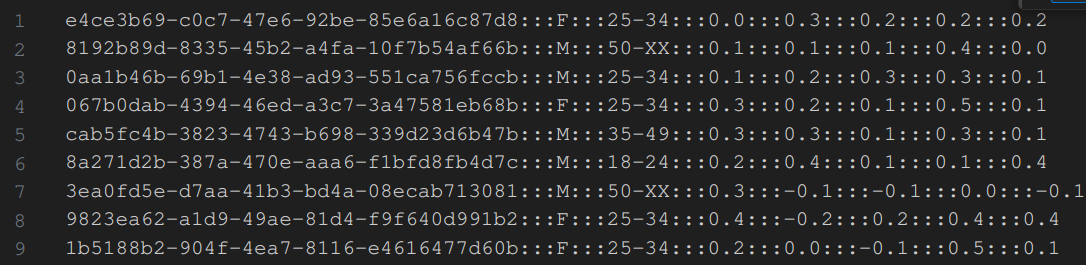
\includegraphics[width=\textwidth]{imaxes/formato_dataset.png}
  \caption{Formato archivo truth.txt \textit{dataset} 2015.}
  \label{fig:formato-dataset}
\end{figure}

  \subsection{PAN author profiling 2016}
  \label{subsec:dataset2016}
  
 Por otra parte, el conjunto de 2016 incluía una partición de entrenamiento formada por textos sacados de usuarios de Twitter y una partición de test formada por texto sacados de Blogs. Estos últimos utilizan un lenguaje más formal, habitualmente conteniendo poemas, canciones o fragmentos de texto no escritos por los usuarios etiquetados que podían afectar negativamente al rendimiento del algoritmo de perfilado. Por estas razones, se decidió utilizar únicamente la partición de entrenamiento para entrenar nuestro clasificador.
 
 El formato de este corpus es bastante similar al del 2015: cada autor aparece representado en un archivo \acrshort{xml} nombrado con un identificador único a partir del cual se puede sacar sus datos demográficos a partir del \gls{ground-truth}.
 
 La diferencia con el de 2015, está en que en vez de aparecer los \textit{tweets} directamente en el \acrshort{xml}, aparecen las URLs a esos \textit{tweets}. Habiendo hasta 1000 URLs por autor. Para conseguir los textos correspondientes a los \textit{tweets} el PAN proporciona un programa\footnote{\url{https://github.com/pan-webis-de/pan-code/tree/master/clef16/author-profiling/twitter-downloader}} que los descargaba y escribía directamente el texto de los mismos en los \acrshort{xml}. Sin embargo, desde 2020 la API de Twitter cambió y este programa dejó de funcionar\footnote{Enlace al \textit{issue} de Github donde lo indican: \url{https://github.com/pan-webis-de/pan-code/issues/3}}.
 
 Por este motivo, se decidió crear un \gls{web-scraper} que fuera leyendo las direcciones URL de los \acrshort{xml} que se correspondían con los \textit{tweets} de los usuarios y descargara el texto de estos sin necesidad de usar la API de Twitter. Sin embargo, este proceso era mucho más lento que el uso del programa antes mencionado (1000 \textit{Tweets}/minuto frente a aproximadamente 30 \textit{Tweets}/minuto). Esto hizo que decidiera emplear la plataforma de Kaggle\footnote{\url{https://www.kaggle.com/}}, para ejecutar diariamente este programa en forma, de manera \textit{serverless}. Kaggle, es una web que permite programar ejecuciones asíncronas de hasta 10 \textit{Jupyter notebooks} concurrentemente, con un límite de 12 horas de duración. Así se descargó el grueso de publicaciones del \textit{dataset}, excepto aquellas pertenecientes a \textit{tweets} y usuarios eliminados. En la figura \ref{fig:scraper}, se muestra una captura de los \textit{logs} resultantes de una ejecución de 12 horas del \textit{scraper} para obtención de estos \textit{tweets}.
 %En total hay 187995 tweets y 843.0269058295964 tweets por autor de media

 \noindent\begin{figure}[hp!]
  \centering
    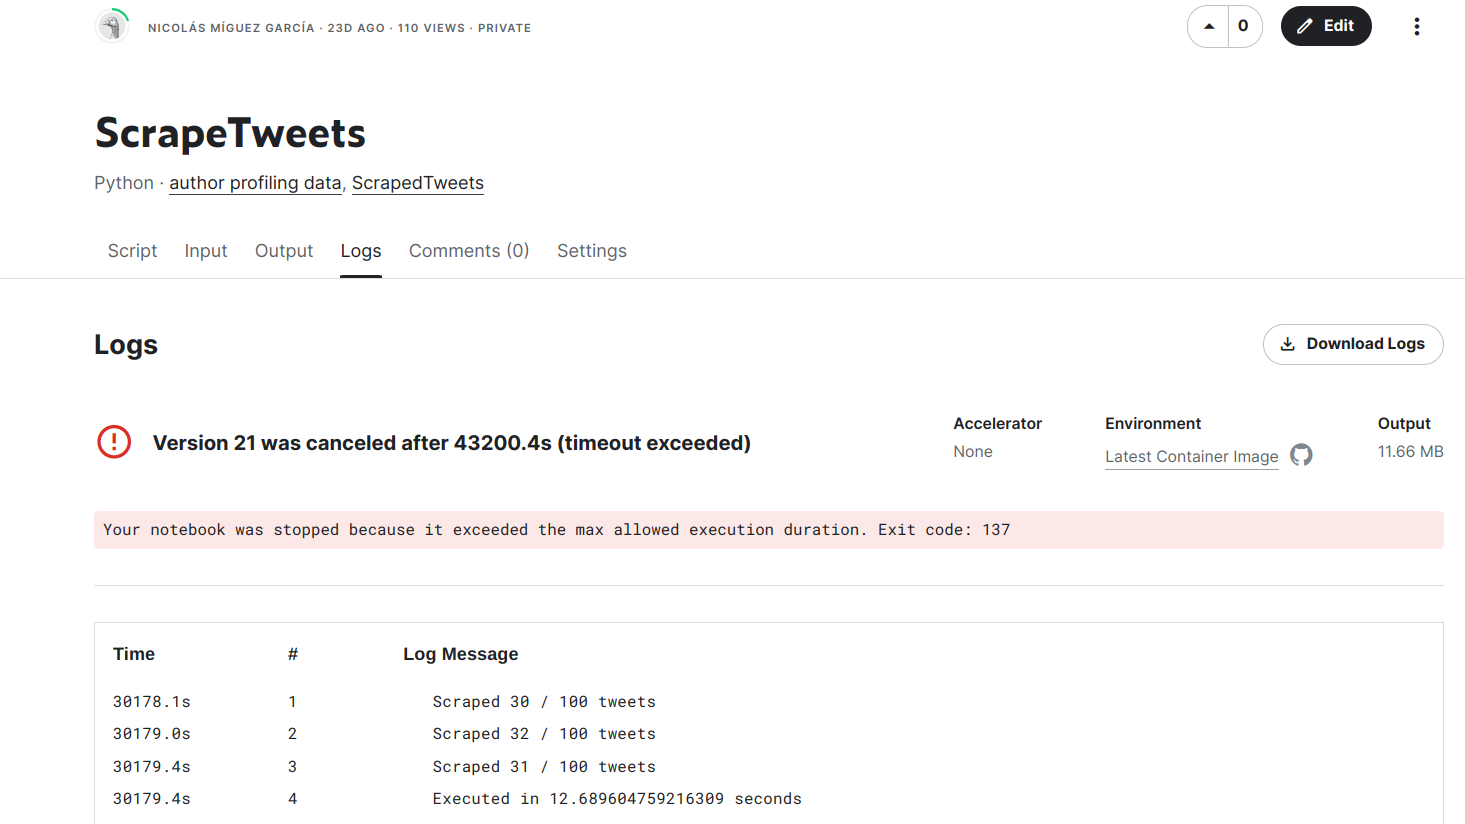
\includegraphics[width=\textwidth]{imaxes/scraper.png}
  \caption{\textit{Logs} resultado de una ejecución del notebook a modo de \textit{scraper} para la obtención de los \textit{tweets} del \textit{dataset} de 2016.}
  \label{fig:scraper}
\end{figure}
 
   \subsection{Distribución de usuarios de los \textit{dataset}}

   En la tabla \ref{tab:datasets_edad}, podemos ver la distribución final de autores en función de edad y género de ambos conjuntos. Como se puede observar los \textit{datasets} están equilibrados en cuestión de género, mientras que están bastante más desequilibrados en cuestión de edad.
   
   Vale la pena mencionar que aunque en el \textit{dataset} de 2016, inicialmente había 250 autores de \textit{Training}, al descargar los textos correspondientes a estos muchos de ellos no estaban disponibles por las razones mencionadas en el apartado anterior~\ref{subsec:dataset2016}. Por lo tanto, descartando estos quedan un total de 222 usuarios.
   
   \begin{table}[hp!]
    \centering
    \rowcolors{2}{white}{udcgray!25}
    \begin{tabular}{|l|ll|l|l|}
        \rowcolor{udcpink!25}
        \hhline{~|---|~}
        \multicolumn{1}{c|}{\cellcolor{white}} & \multicolumn{2}{c|}{\textbf{PAN-AP 2015}} & \textbf{PAN-AP 2016} & \multicolumn{1}{c}{\cellcolor{white}}\\ \hhline{-----|}
        Categoría & Training & Test & Training & Total\\ \hline
        18-24 & 22 & 18 & 11 & 51\\
        25-34 & 46 & 44 & 54 & 144\\
        35-49 & 22 & 18 & 116 & 156\\
        +50 & 10 & 8 & 41 & 59\\ \hline
        Hombres & 50 & 44 & 111 & 204\\
        Mujeres & 50 & 44 & 111 & 204\\ \hline
        Total & 100 & 88 & 222 & 410\\ \hline  
    \end{tabular}%
    \caption{Distribución de usuarios en función de edad y género en los conjuntos de entrenamiento utilizados.}
    \label{tab:datasets_edad}
\end{table}

\section{Búsqueda y comparación de algoritmos}

En esta sección, se detalla la fase del proyecto consistente en 
 la investigación sobre los algoritmos y modelos existentes de clasificación de texto para tareas de perfilado automático de usuarios.
 
 El objetivo principal de esta fase era el análisis del estado del arte en este campo con la finalidad de escoger y replicar los algoritmos de perfilado de usuarios más robustos para nuestro trabajo. En consecuencia, vale la pena resaltar que la intención no era crear un algoritmo de perfilado original a partir de cero, sino emplear uno ya implementado, del que se tenga conocimiento que reporta buenos resultados.
 
 Para ello, se orientó la búsqueda hacia las competiciones ya mencionadas en el apartado \ref{sec:estado_arte} como PAN \citep{pan:2013} o IberLef \citep{iberlef2022}. Esto tiene dos motivos: primero que seleccionando los algoritmos de entre los participantes en una de estas competiciones, contamos con la información previa de la bondad de los algoritmos con los otros competidores, pudiendo así seleccionar los que mejor se comportaron en las mismas; por otra parte, al ser competiciones abiertas al público, es más sencillo encontrar de forma pública las implementaciones de los algoritmos de participantes en repositorios como Github\footnote{\url{https://github.com/}}.
 
En la tabla \ref{tab:comparacion-profilers}, se muestra una pequeña comparativa de los algoritmos del estado del arte con implementación disponible en Github. En ella se tiene en cada columna: la referencia a las \textit{working notes} del equipo participante de la tarea, la competición para la que se desarrolló, la posición final en la que quedó el equipo participante (teniendo en cuenta perfilado en idioma español solamente), las resultados alcanzados en términos de \textit{accuracy} o precisión para edad y género en la competición en la que participaron, el modelo de aprendizaje automático utilizado y un resumen muy general de las características extraídas para la clasificación del texto.

Como se puede ver en ella muchos de estos algoritmos usan modelos y características bastante similares entre ellos. En consecuencia, solo se decidieron replicar aquellos tres que fueran menos similares entre sí \citep{loscalis22, modaresi:2016, grivas2015author}.


\begin{table}[H]
    \centering
    \rowcolors{2}{white}{udcgray!25}
    {
    \setlength{\tabcolsep}{0.2\tabcolsep}
        \begin{tabular}{|p{0.13\linewidth} |p{0.17\linewidth} |p{0.04\linewidth} |p{0.07\linewidth} |p{0.09\linewidth} |p{0.09\linewidth} | p{0.2\linewidth} |}
            \hline
            \rowcolor{udcpink!25}
            
            \textbf{Equipo} & \textbf{Competición}  & \textbf{\#} & \textbf{Edad} (Acc) & \textbf{Género} (Acc) & \textbf{Modelo} & \textbf{Características}\\ \hline
            \citet{grivas2015author} & PAN 2015 \citep{pan:2015} & 3º & 0.7465 & 0.8592 & \gls{svm} & Tfidf n-grams stylistic features\\
            \citet{modaresi:2016} & PAN 2016 \citep{pan:2016} & 2º & 0.5179 & 0.6964 & \gls{lr} & Tfidf n-grams stylistic features\\
            \citet{Daneshvar2018} & PAN 2018 \citep{pan:2018} & 1º & -- & 0.8200 & \gls{svm} & Tfidf n-grams + LSA\\
            \citet{bacciu2019bot} & PAN 2019 \citep{pan:2019} & 3º & -- & 0.7761 & \gls{svm} & Tfidf n-grams + LSA\\
            Baseline & PAN 2020 \citep{pan:2020} & & 0.6310 & 0.5000 & \gls{lr} & Tfidf n-grams\\
            \citet{loscalis22} & IberLef 2022 \citep{iberlef2022} & 1º & -- & 0.9029 & \gls{mlp} & Embeddings (BERT + RoBERTa)\\
            \citet{holgado2022halbert} & IberLef 2022 \citep{iberlef2022} & 5º & -- & 0.7260 & \gls{em} & n-grams + embeddings + stylistic features\\ \hline
        \end{tabular}
    }
    \caption{Comparación de algoritmos del estado del arte en perfilado de usuarios de los cuales se encontró la implementación disponible en Github.}
    \label{tab:comparacion-profilers}
\end{table}

\subsection{Primera aproximación}
\label{subsec:1aprox}

En primer lugar, tenemos al ganador de la competición del IberLef 2022 \citep{iberlef2022}. Esta competición consistía en la predicción de género, profesión e ideología política, binaria (izquierda y derecha) y multiclase (izquierda, centro-izquierda, centro-derecha y derecha), de usuarios de Twitter sobre un corpus de \textit{tweets} procedentes de periodistas, políticos y españoles.

En ella, la mayoría de aproximaciones empleadas, consistían en modelos basados en \textit{transformers} \citep{vaswani2017attention}. Los cuales son grandes modelos de lenguaje pre-entrenados (BETO \citep{BETO}, MarIA \citep{MarIA}, BERT multilingüe, ALBERT\dots) afinados con el corpus de la competición, con el objetivo de extraer características del texto a nivel de documento. Este tipo de arquitecturas, basadas en \textit{transformers}, son la gran novedad con respecto a los enfoques utilizados en competiciones de años anteriores del PAN.

%%%%%%%%%%%%%%%%%%%%%%%%%%%%%%%%%%%%%%%%%%%%%%%%%%%%%%%%%%%
% \subsubsection{Transformers y modelos de lenguaje}
% TODO 
% meter teoría sobre transformers y modelos de lenguaje
%%%%%%%%%%%%%%%%%%%%%%%%%%%%%%%%%%%%%%%%%%%%%%%%%%%%%%%%%%%

El enfoque utilizado por \citet{loscalis22} por tanto, combinaba el modelo BERT \citep{devlin2019bert} pre-entrenado en idioma español, conocido como BETO \citep{BETO} junto con el modelo RoBERTa pre-entrenado también en español, llamado MarIA \citep{MarIA}. Este emplea ambas arquitecturas para extracción de características a nivel de documento y en base a estas se entrena un perceptrón multicapa para decodificar las etiquetas de los usuarios. En la figura \ref{fig:arquitectura} se muestra la arquitectura del modelo utilizado.

\noindent\begin{figure}[hp!]
  \centering
    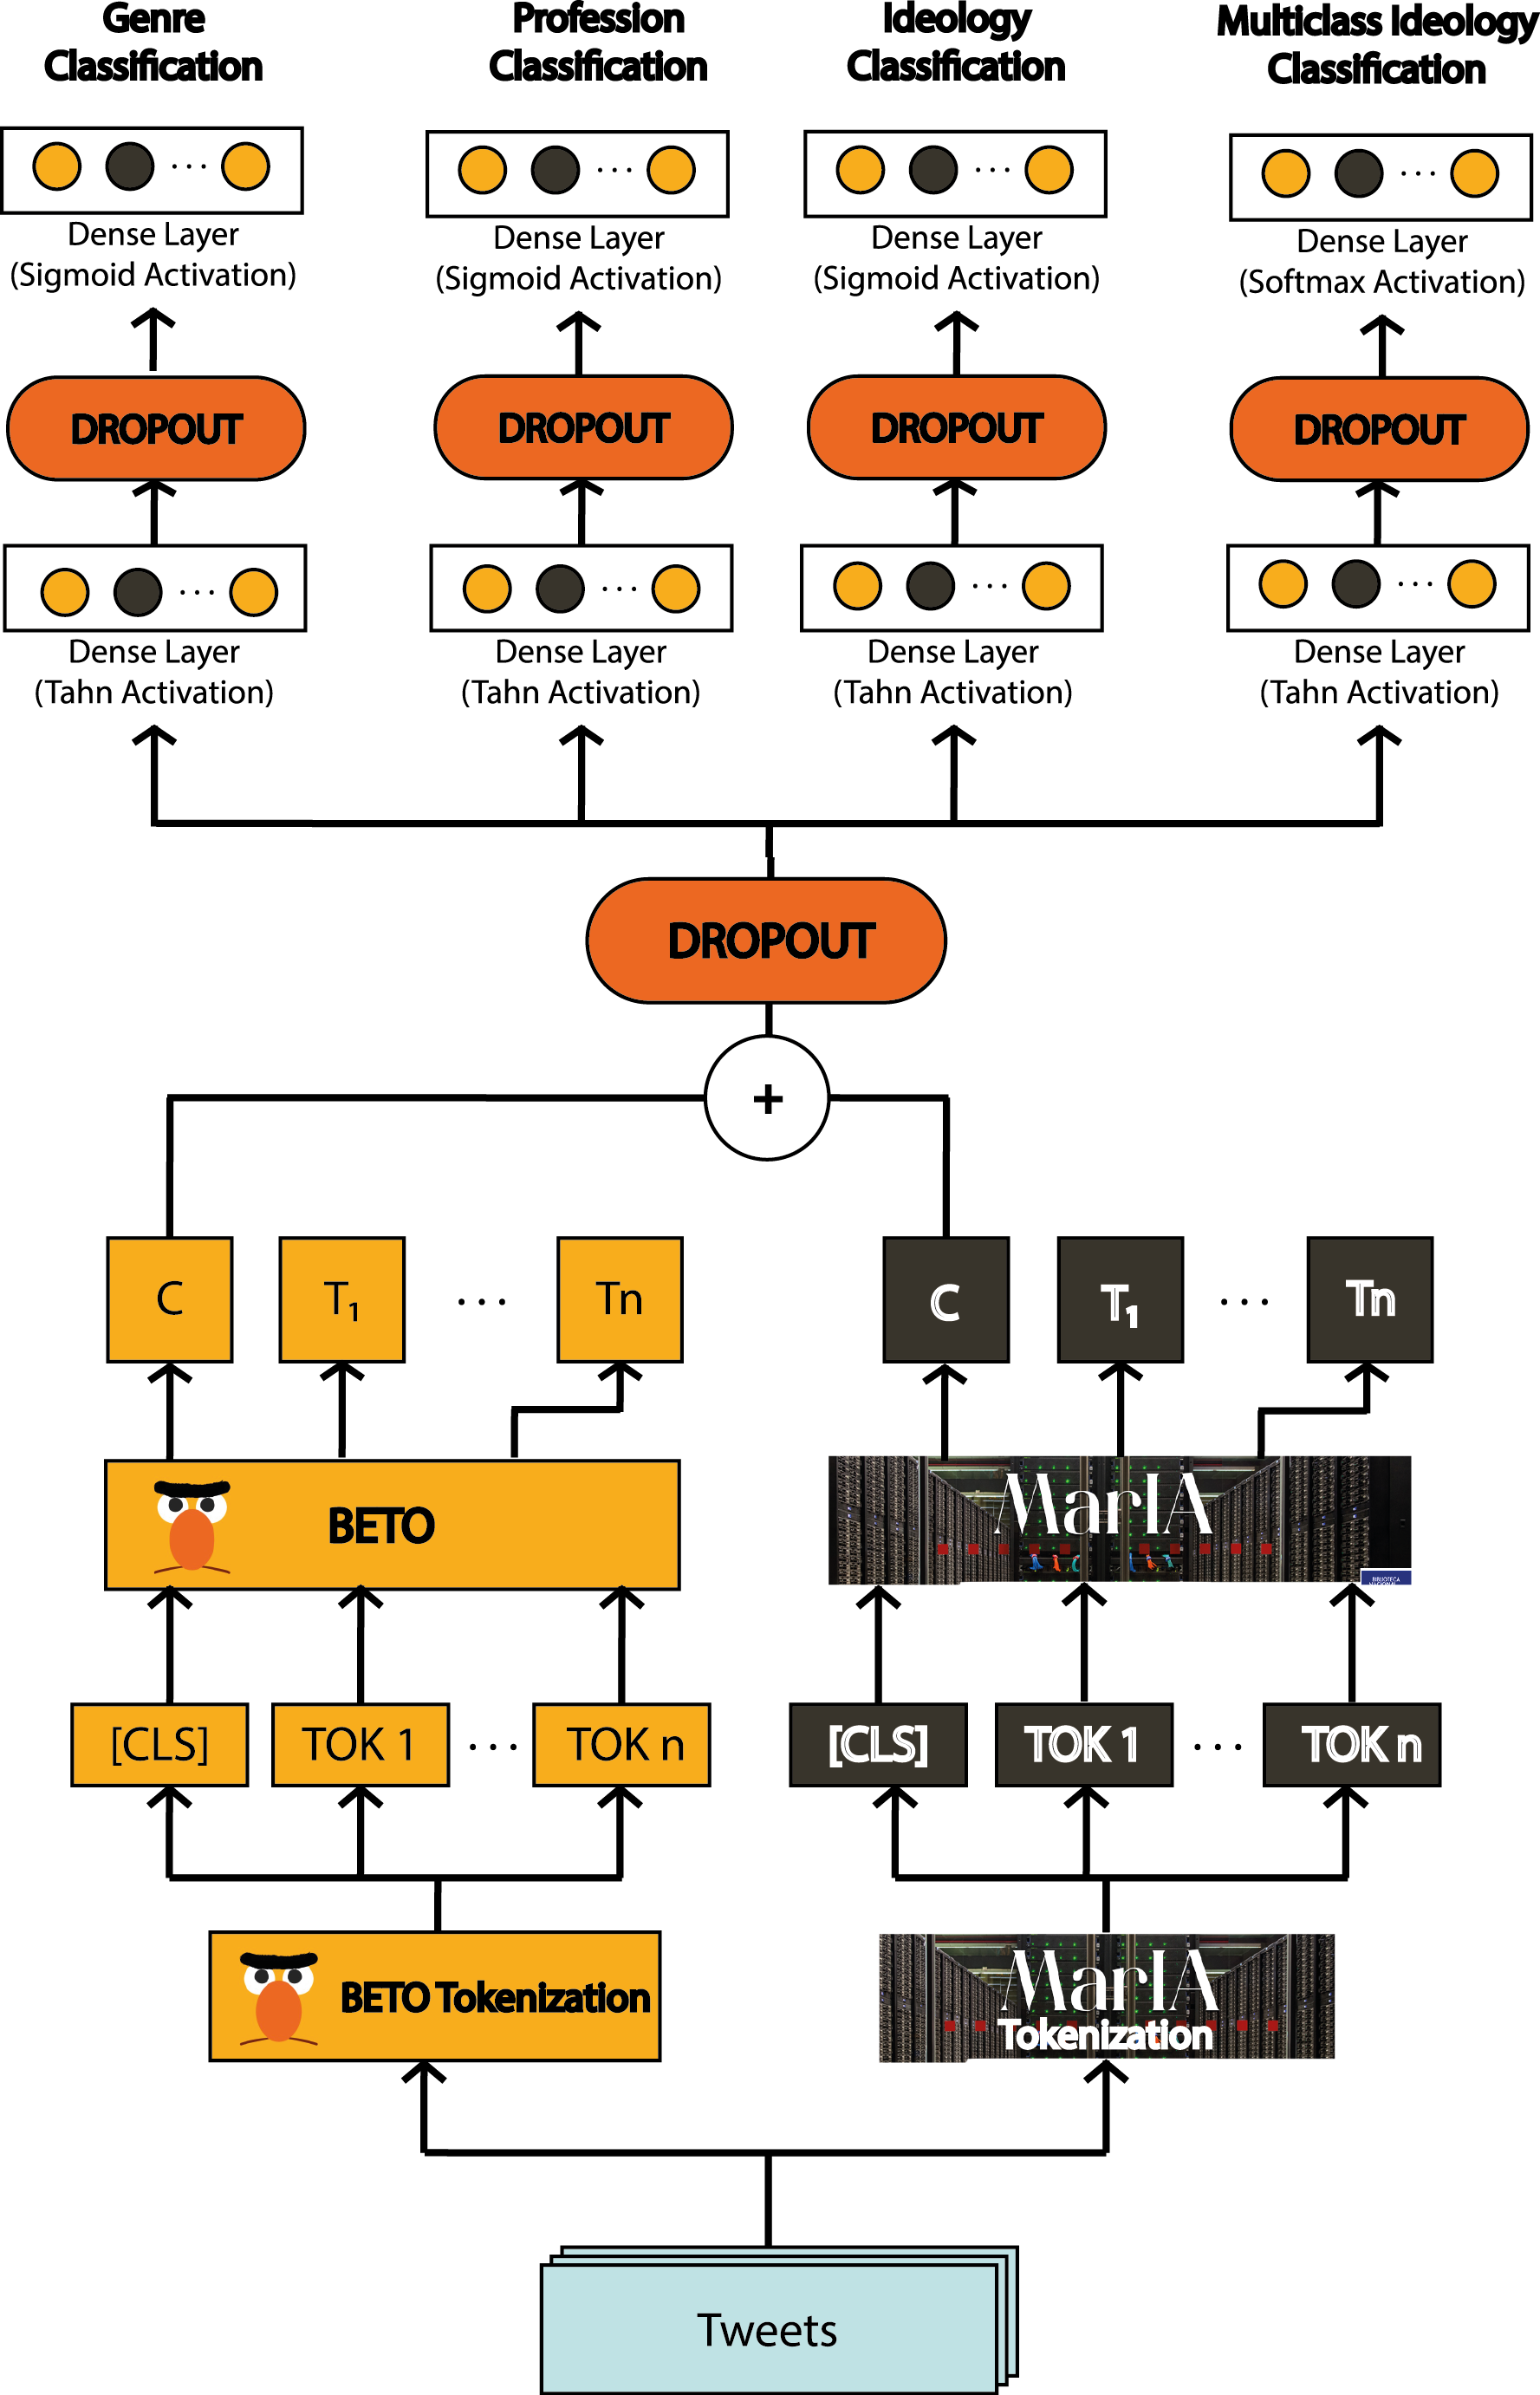
\includegraphics[height=0.8\textwidth]{imaxes/arquitectura_.png}
  \caption{Arquitectura del modelo ganador de la competición de Political Author Profiling del IberLef 2022, utilizado por \citet{loscalis22}.}
  \label{fig:arquitectura}
\end{figure}

\subsubsection{Preprocesado}

Por una parte, está el preprocesado realizado a la hora de la creación del corpus por los organizadores de la competición. Este consistió en descartar \textit{retweets}, \textit{tweets} donde se parafrasean titulares de periódicos o \textit{tweets} en otros idiomas distintos del español. Además de esto, se anonimizó la colección sustituyendo las menciones a usuarios por el token "@user".

Por otro lado, el preprocesado efectuado por \citet{loscalis22} se limitó a la agrupación de los \textit{tweets} de un mismo autor en bloques de máximo 512 tokens tras la \textit{tokenización} con BERT y RoBERTa. Esto es así debido a que los modelos basados en BERT no aceptan entradas de mayor tamaño.

En nuestro caso, se realizó un preprocesado parecido con la excepción de que se mantuvieron todos los \textit{tweets} de la colección aunque contuvieran fragmentos en otros idiomas o parafrasearan titulares de noticias o blogs. La razón de esto es que nuestros \textit{datasets} de entrenamiento cuentan con un volumen mucho menor de textos en relación a los corpus de la competición del IberLef, por ello creímos preferible no realizar esa limpieza para mantener un corpus lo más grande posible.

Por otro lado, también se optó por sustituir las URLs encontradas por el token '<URL>', debido a que en el corpus de la competición no se incluían estas tampoco. Además, se optó por sustituir los emoticonos encontrados en el texto por el token '<EMOTICON>' y los emojis por su descripción sacada de la librería emoji\footnote{\url{https://pypi.org/project/emoji/}}.

\subsubsection{Modelo}
En nuestro caso se replicó el mismo modelo usado por los participantes de la tarea, únicamente adaptando las salidas de la red. En el caso de \citet{loscalis22}, tenían tres salidas binarias (género, profesión, ideología binaria) y una multiclase (ideología multiclase). En nuestro problema, se tienen únicamente dos salidas: género y edad. En consecuencia se utilizó la arquitectura que se puede ver en la figura \ref{fig:arquitectura_adaptada}. En ella se muestra que se mantienen las mismas capas y funciones de activación que en la arquitectura original con la diferencia de que en vez de cuatro bloques separados de decodificación de las etiquetas, ahora tenemos únicamente dos.

\noindent\begin{figure}[H]
  \centering
    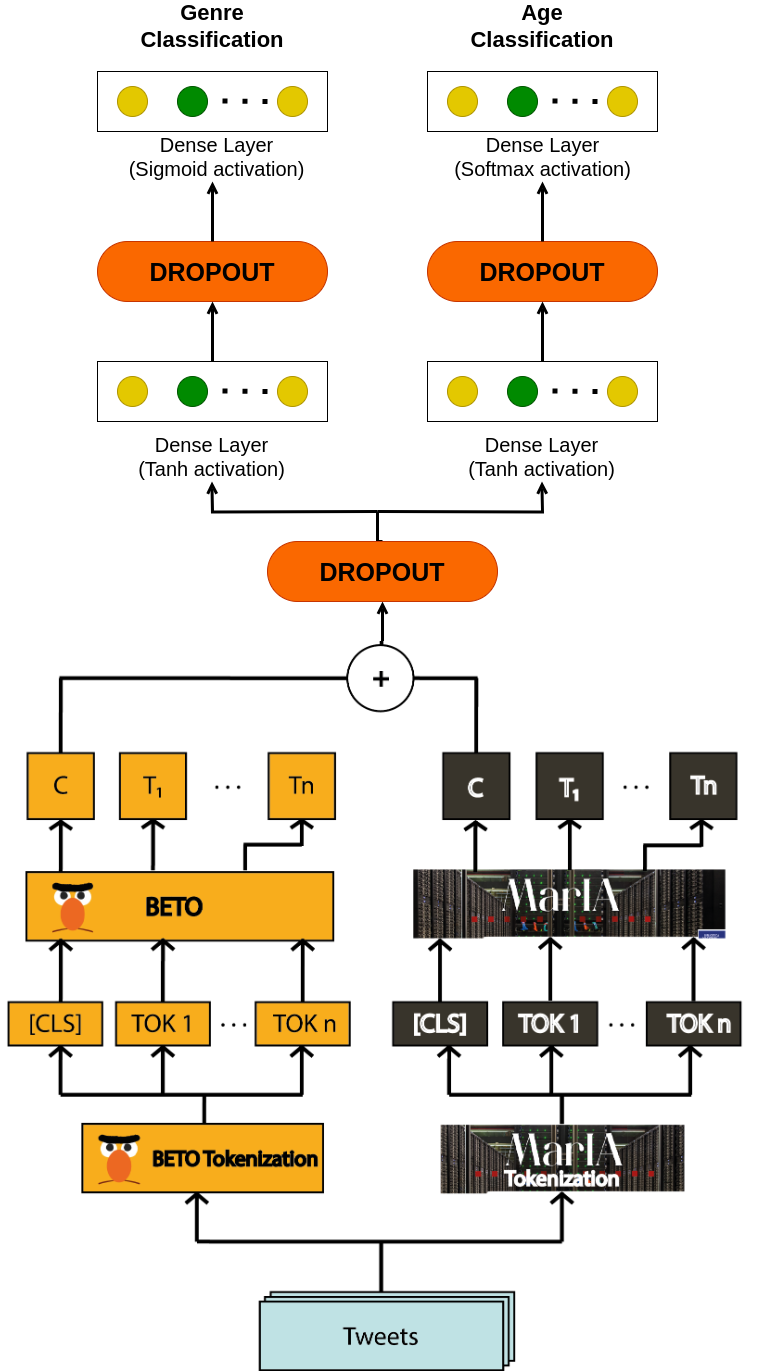
\includegraphics[height=0.8\textwidth]{imaxes/diagrama_arquitectura_profiler.png}
  \caption{Arquitectura basada en transformers adaptada de la aproximación de \citet{loscalis22}.}
  \label{fig:arquitectura_adaptada}
\end{figure}

\subsubsection{Métricas}
\label{subsubsec:metricas}
Como métricas para estos experimentos, se decidió utilizar por una parte, la precisión (\textit{\textbf{accuracy}} en inglés), que se calcula de acuerdo a la fórmula \ref{eq:acc}. El motivo es principalmente que es la métrica usada en las competiciones PAN, por ello, es ideal para comparar los resultados con los obtenidos por los propios autores en la competición de referencia. Esta es una buena opción, cuando se tienen clases bien balanceadas, como es nuestro caso con el género de los ususarios, además proporciona una medida de rendimiento general del modelo.


\begin{equation}
  \text{\textit{Accuracy}} = \frac{\text{Predicciones correctas}}{\text{Predicciones totales}}
  \label{eq:acc}
\end{equation}

Por otro lado, se optó además por usar la \textbf{F1 ponderada} (\textit{weighted} en inglés). La F1 es una métrica adecuada cuando se quiere dar igual importancia tanto a la sensibilidad como la especificidad del modelo, para una clase se calcula como en la fórmula \ref{eq:f1}. Al realizar la media de la F1 de cada clase, ponderada por el número de instancias de cada clase (fórmula \ref{eq:f1w}), esta no se ve afectada por el desbalance entre clases del conjunto de datos, lo cual es ideal para tratar con el desequilibrio en cuestión de edad (\hyperref[tab:datasets_edad]{conjunto de datos}). 

\begin{equation}
    F1 = 2 \cdot \frac{\text{Sensibilidad} \cdot \text{Especificidad}}{\text{Sensibilidad} + \text{Especificidad}}
      \label{eq:f1}
\end{equation}

\begin{equation}
    F1_{\text{weighted}} = \frac{\sum_{i} w_i \cdot F1_i}{\sum_{i} w_i}
  \label{eq:f1w}
\end{equation}

\subsubsection{Experimentos realizados}
Se realizaron distintas pruebas con los conjuntos de datos expuestos en la sección \ref{sec:datasets}. Para estas se utilizaron la misma configuración de hiper-parámetros propuesta por \citet{loscalis22}, que se puede ver en la tabla \ref{tab:hiperparametros}. 

\begin{table}[hp!]
    \centering
    % \rowcolors{2}{white}{udcgray!25}
    \begin{tabular}{ll}
        \hline
        % \rowcolor{udcpink!25}
        \textbf{Parámetro}  & \textbf{Valor} \\ \hline
        Train batch size    & 64             \\
        Predict batch size  & 8              \\
        Learning rate       & 3e-5           \\
        Training epochs     & 5              \\
        Max sequence lenght & 512            \\
        Dropout             & 0.15           \\
        Optimizer           & Adam           \\
        Dense layer units   & 768            \\ \hline
    \end{tabular}
    \caption{Hiperparámetros utilizados en los experimentos, propuestos por \citet{loscalis22}.}
    \label{tab:hiperparametros}
\end{table}
En la tabla \ref{tab:resultados-bert} se pueden ver los experimentos realizados así como los resultados obtenidos en cada uno de ellos en términos de \textit{accuracy} y F1-\textit{weighted} para género y edad.

\begin{table}[H]
    \centering
    \rowcolors{2}{white}{udcgray!25}
    {
    \setlength{\tabcolsep}{0.6\tabcolsep}
        \begin{tabular}{|l|l|ll|ll|}
            \hline
            \rowcolor{udcpink!25}
            \multicolumn{2}{|c|}{\textbf{\textit{Dataset}}} & \multicolumn{2}{c|}{\textbf{Género}} & \multicolumn{2}{c|}{\textbf{Edad}} \\ \hline
            \textbf{Entrenamiento} & \textbf{Test} & \textbf{Acc} & \textbf{F1-w} & \textbf{Acc} & \textbf{F1-w}\\ \hline
            Training 2015     & Test 2015         & 0.8863   & 0.8863 & 0.6250   & 0.6104\\
            2015 (Train+Test) & Training 2016     & 0.4865 & 0.3907 & 0.2703     & 0.1716\\
            Training 2016     & 2015 (Train+Test) & 0.4468   & 0.4324 & 0.3191   & 0.3092\\
            Training 2016     & Test 2016         & 0.4545   & 0.4509 & 0.4181   & 0.3601\\ \hline
        \end{tabular}
    }
    \caption{Resultados para género y edad en distintos experimentos, utilizando el enfoque propuesto por \citet{loscalis22} con las particiones de entrenamiento y test de las competiciones de PAN de 2015 y 2016.}
    \label{tab:resultados-bert}
\end{table}

Lo primero que llama la atención de estos, es la diferencia de rendimiento obtenida usando el \textit{dataset} de 2015, a modo de réplica de la competición del PAN \citep{pan:2015}, con el resto de experimentos realizados.

En el primer caso los resultados no se alejan demasiado de los conseguidos por el equipo ganador de la misma: 0.9659 y 0.7955, para género y edad respectivamente.

Sin embargo, cuando se trata de aumentar estos datos para obtener mejores resultados, por ejemplo usando el \textit{dataset} completo de 2015 (entrenamiento y test) para entrenar el modelo y se prueban a predecir los autores del corpus de entrenamiento del 2016 se puede ver como los resultados obtenidos empeoran considerablemente, hasta el punto de ser peores que un clasificador aleatorio. Esto se repite al entrenar con la partición de \textit{Training} de 2016 y testear con la de 2015 completa o con la de Test de 2016 (competición PAN 2016).

Para solventar este problema, lo primero que se intentó fue separar una parte del conjunto de entrenamiento para usarlo como conjunto de validación, con la finalidad de observar como se comportaba la función de pérdida de la red.

%\footnote{La función de pérdida, conocida simplemente como \textit{loss}, es una medida que se utiliza para cuantificar la bondad de un modelo (típicamente una red neuronal) de forma que sirva de guía a la hora de optimizar los parámatros (pesos) del mismo durante el proceso de entrenamiento, con el objetivo de minimazar el valor de la misma.}

La función de pérdida o (\textit{loss} en inglés) en aprendizaje automático mide la discrepancia entre la clasificación de las predicciones de la red y los datos reales. En las redes neuronales, el objetivo del entrenamiento consiste en la minimización del valor de esta función en cada ciclo mediante del ajuste del valor de los pesos de las conexiones de la red, por medio del algoritmo de retro-propagación del error. Como se explica en \citet{janocha2017loss}, existen diversas alternativas a la hora de escoger una función de pérdida, sin embargo, para problemas de clasificación es bastante común el uso de la entropía cruzada (pérdida logarítmica), por lo cual es la elegida para nuestro algoritmo.

De esta forma viendo la evolución del \textit{loss} durante el entrenamiento, se podría saber si el sistema estaba sobre-entrenado o no. Pues bien, los resultados de esta prueba se pueden ver en la figura \ref{fig:loss}.

 \begin{figure}[H]
    \centering
    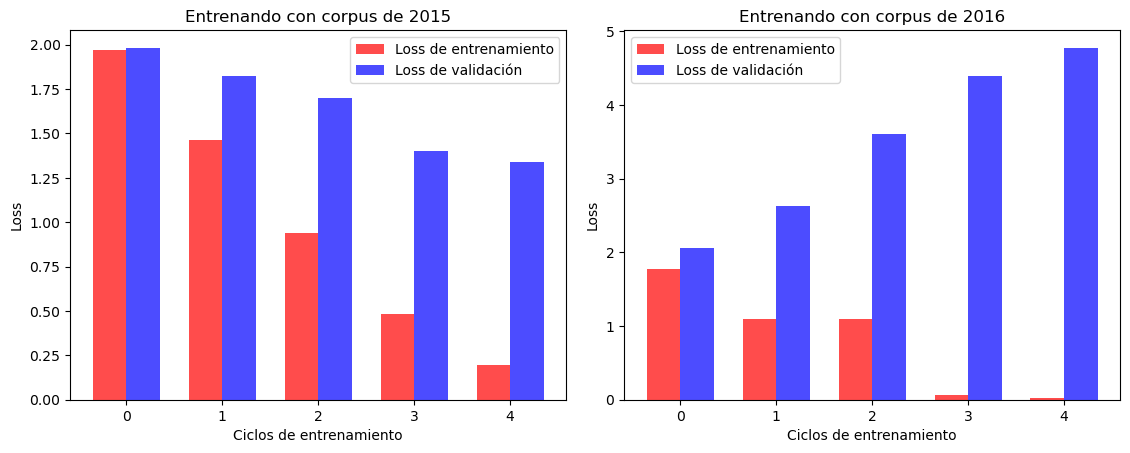
\includegraphics[width=\textwidth]{imaxes/loss.png}
    \caption{Evolución del loss de entrenamiento y validación del modelo propuesto por \citet{loscalis22} al entrenar con los \textit{datasets} de 2015 y 2016.}
    \label{fig:loss}
\end{figure}

Como se puede ver, a la hora de entrenar el modelo con los datos de 2015 el \textit{loss} del conjunto de validación disminuía al mismo tiempo que el \textit{loss} del conjunto de entrenamiento; sin embargo, a la hora de entrenar usando el corpus de entrenamiento de 2016 pasaba justo lo contrario, el \textit{loss} de validación aumentaba cada ciclo mientras el de entrenamiento disminuía (signo de que el modelo se está sobre-ajustando a los datos de entrenamiento y no consigue generalizar).

 Tras descubrir esto, lo primero que se me ocurrió fue investigar un poco los dos conjuntos y compararlos para descubrir si existía alguna diferencia entre ellos. Lo que se descubrió fue que probablemente en el \textit{dataset} de 2015, tanto en el conjunto de entrenamiento como en el de test existían autores repetidos, de modo que el modelo obtenía buenos resultados debido a que el modelo se aprendía el las características textuales de usuarios concretos y no a distinguir la edad o género de una persona aleatoria.
 
 Por otro lado, la diferencia de rendimiento entre el modelo adaptado a nuestro problema y el propuesto por \citet{loscalis22} se especula que se deba probablemente a el mayor tamaño del corpus usado para entrenar en la competición del IberLef (alrededor de 400.000 \textit{tweets} de más de 700 usuarios distintos, frente a 222 usuarios con aproximadamente 800 \textit{tweets} cada uno) unido a un vocabulario más formal usado por políticos y periodistas españoles junto a unas temáticas mucho más menos variadas, comparado con el vocabulario del usuario promedio de Twitter lleno de expresiones de jerga, abreviaturas y disparidad de temáticas tratadas.
 
 Debido a estos malos resultados obtenidos y a la falta de un corpus de mayor tamaño necesario para entrenar un modelo complejo basado en aprendizaje profundo, se decidió orientar el trabajo hacia modelos más sencillos como los expuestos a continuación.

\subsection{Segunda aproximación}
\label{subsec:2aprox}

Por otro lado el segundo algoritmo de perfilado probado es el correspondiente a \citet{grivas2015author}. Este obtuvo la tercera posición general en la tarea de author profiling de PAN 2015~\citep{pan:2015}.

Los \textit{\textbf{datasets}} usados en aquella tarea son los explicados en la subsección \ref{subsec:pan15}.

\subsubsection{Preprocesado}
El preprocesado realizado es distinto dependiendo del tipo de características extraídas. Así los autores de este trabajo separan por un lado características estructurales y características estilométricas.

Las primeras incluyen el numero de menciones, \textit{hashtags} y URLs que contienen los \textit{tweets}. Las segundas, se refieren a la longitud del \textit{tweet} en caracteres y tf-idf n-grams.

Para las estructurales no se realizó ningún preprocesado del texto a parte de concatenar todos los \textit{tweets} de un autor. Por otro lado, para las estilométricas se eliminaron: etiquetas HTML, URLs, menciones, así como los caracteres '\#' de los \textit{hashtags}.

\subsubsection{Modelo}
Para la clasificación del género, se usó una \gls{svm} con kernel rfb, y se usaron como características únicamente los tf-idf n-grams. En cuanto a la edad, se usó una \gls{svm} con kernel linear a la que se le pasaron como características: tf-idf ngrams, longitud del \textit{tweet}, número de URLs, menciones y \textit{hashtags}. Además, se compensó el desbalanceo de los distintos grupos de edad mediante pesos inversamente proporcionales a la frecuencia de las clases.

\subsubsection{Experimentos y resultados}
En la tabla \ref{tab:aprox2_results} se pueden observar los resultados de los experimentos realizados en esta aproximación. Las métricas elegidas tanto para género como edad son las mismas que en la anterior (\hyperref[subsubsec:metricas]{métricas}).

\begin{table}[H]
    \centering
    \rowcolors{2}{white}{udcgray!25}
    \resizebox{\textwidth}{!}{%
    \setlength{\tabcolsep}{0.3\tabcolsep}
    \begin{tabular}{|l|ll|ll|ll|}
        \hhline{~|------}
        \rowcolor{udcpink!25}
        \multicolumn{1}{c}{\cellcolor{white}} & \multicolumn{2}{|c|}{\textbf{\textit{Dataset}}} & \multicolumn{2}{c|}{\textbf{Género}} & \multicolumn{2}{c|}{\textbf{Edad}} \\ \hline
        \textbf{N-gram} & \textbf{Entrenamiento} & \textbf{Test} & \textbf{Acc} & \textbf{F1} & \textbf{Acc} & \textbf{F1} \\ \hline
        Carácter [3, 3] & Training 2015 & Test 2015 & 0.9091 & 0.9089 & \textbf{0.7159} & \textbf{0.7098} \\
        Carácter [3, 5 ] & Training 2015 & Test 2015 & \textbf{0.9205} & \textbf{0.9202} & 0.6932  & 0.6835 \\ \hline
        Carácter [3, 3] & Training 2015 & Training 2016 & 0.5818 & \textbf{0.5427} & \textbf{ 0.3423}  & \textbf{ 0.2782} \\
        Carácter [3, 5] & Training 2015 & Training 2016 & \textbf{0.5856} & 0.5338 & 0.3018  & 0.2309\\ \hline
        Carácter [3, 3] & 2015 (Train+Test) & Training 2016 & 0.5405 & 0.4501 & \textbf{0.3468}  &\textbf{ 0.2987} \\
        Carácter [3, 5] & 2015 (Train+Test) & Training 2016 & \textbf{0.5586} & \textbf{0.4621} & 0.2972  & 0.2253 \\ \hline
        Carácter [3, 3] & Training 2016 & 2015 (Train+Test) & 0.5638 & 0.5386 & 0.4627  & 0.3878 \\ \hline
        Carácter [3, 3] & Training 2016 & Test 2016 & 0.5091 & 0.3435 & 0.4545  &  0.4195 \\ \hline
        Carácter [3, 3] & Training 2016 & *10-Fold CV & 0.6712 & 0.6692 & \textbf{0.5045}  & \textbf{0.3739}\\
        Carácter [3, 5] & Training 2016 & *10-Fold CV & 0.6757 & 0.6746 & \textbf{0.5045}  & 0.3739 \\
        Carácter [5, 8] & Training 2016 & *10-Fold CV & 0.6667 & 0.6707 & 0.4945  & 0.3593\\
        Palabra  [1, 3] & Training 2016 & *10-Fold CV & \textbf{0.6937} & \textbf{0.6750} & 0.4910  & 0.3705 \\ \hline
        Carácter [3, 3] & 2015+2016 (Train) & *10-Fold CV & 0.7024 & 0.6960 & 0.6073  & 0.5657 \\
        Carácter [3, 5] & 2015+2016 (Train) & *10-Fold CV & \textbf{0.7170} & \textbf{0.7133} & 0.5707  & \textbf{0.5747} \\
        Carácter [5, 8] & 2015+2016 (Train) & *10-Fold CV & \textbf{0.7170} & 0.7128 & \textbf{0.6195}  & 0.5178 \\
        Palabra  [1, 3] & 2015+2016 (Train) & *10-Fold CV & 0.6610 & 0.6583 & 0.5390  & 0.4674 \\
        Palabra  [1, 1] & 2015+2016 (Train) & *10-Fold CV & 0.7122 & \textbf{0.7113} & 0.5829  & 0.5355 \\\hline
        \end{tabular}%
    }
    \caption{Resultados en términos de precisión para género y edad de los experimentos realizados para la aproximación 2 (modelo propuesto por \citet{grivas2015author}).}
    \label{tab:aprox2_results}
\end{table}

Una vez más sucede que los resultados obtenidos de replicar la competición del PAN 2015, son mucho mejores que el resto de experimentos realizados, lo que afianza la teoría de que en ese \textit{dataset} existen autores repetidos, es decir, no hay independencia entre \textit{Training} y Test.

Por otro lado, esta aproximación reporta mejores resultados tanto en género como en edad en el resto de experimentos realizados. Por ejemplo, al entrenar con el \textit{dataset} de 2016 y hacer test con 2015 el \textit{profiler} ya es ligeramente mejor que un clasificador aleatorio: 56\% y 46\% de precisión para género y edad respectivamente. Lo que refuerza la idea de que en caso de disponer de un corpus de tamaño relativamente pequeño los modelos tradicionales más sencillos son preferibles a los grandes modelos de lenguaje basados en aprendizaje profundo y \textit{transformers} que están de moda actualmente.

Los resultados de replicar la competición de PAN 2016 (entrenamiento 2016 y test 2016) muestran como este modelo no generaliza bien a otros géneros a parte de Twitter como son los textos de Blogs, utilizados en el \textit{dataset} de Test de 2016.

Para finalizar, en las últimas filas de la tabla se investigó acerca del tipo de características basadas en n-grams que mejor funcionaban en estos \textit{datasets}. Para ello se utilizó un 10-fold Cross-Validation con el \textit{dataset} de \textit{Training} de 2016 y el \textit{dataset} de \textit{Training} de 2016 sumado al de 2015 completo (\textit{Training} y Test). El cross-validation se utilizó en parte para evitar el sesgo de que pueda haber autores repetidos en los datos del 2015 y porque en 2016 la partición de Test contenía textos de un género distinto (textos de Blogs) que la de entrenamiento. 

Finalmente, respecto a las características usadas se puede afirmar, en general los n-grams basados en secuencias de 3-5 caracteres son los que mejor rendimiento tienen para la predicción de género . Mientras que, los n-grams basados en secuencias de 3 caracteres son las que mejores resultados obtienen para edad. No obstante, el hecho de que entre los rangos probados no haya una diferencia significativa de rendimiento en la clasificación, hace preferible el uso de secuencias más cortas como las de 3 caracteres (las cuales fueron las escogidas en el algoritmo original \citep{grivas2015author}) debido al mejor rendimiento computacional del algoritmo general, pues el uso de secuencias más largas impone una carga computacional importante.

\subsection{Tercera aproximación}
\label{subsec:3aprox}

El último \textit{profiler} analizado es el correspondiente al trabajo de \citet{modaresi:2016}. Este fue propuesto para la competición del PAN 2016 \citep{pan:2016}. En ella los participantes debían realizar un modelo que predijese el género y edad de autores de textos sacados de Blogs\footnote{\url{https://www.blogger.com/about/}} habiendo entrenado el mismo a partir de textos de usuarios de Twitter (\ref{sec:datasets}). Por lo tanto, para el desarrollo del algoritmo se valoró por encima de todo, la independencia del mismo con el género de los textos, lo cual es una tarea parecida a nuestro problema, ya que entrenamos con textos sacados de una red social como Twitter, para predecir usuarios de Reddit.

En esta competición los resultados fueron bastante peores comparados con las anteriores (es probable que en parte sea debido a la dificultad añadida de la misma): el autor de este modelo \citep{modaresi:2016}, el cual quedó en segunda posición en idioma español, obtuvo 0.6964 y 0.5179 para género y edad respectivamente.

\subsubsection{Preprocesado}

El procesado realizado en este algoritmo, tenía la intención de eliminar la información específica de género presente en los textos. Así, se usaron distintas operaciones de preprocesado en función de las características extraídas del texto. A continuación se enumeran estas operaciones:

\begin{itemize}
    \item p1: Pasar el texto a minúsculas.
    \item p2: Filtrar cualquier URL encontrada.
    \item p3: Eliminar menciones en las que aparezca un nombre de usuario del tipo <<@username>>.
    \item p4: Eliminar todos los \textit{Hashtags} del texto.
    \item p5: Eliminar los \textit{retweets} encontrados (en teoría no existen en el \textit{dataset}).
    \item p6: Eliminar cualquier carácter no latino encontrado.
    \item p7: Eliminar acentos latinos de palabras, para favorecer la precisión de características basadas en \textit{n-grams}.
    \item p8: Eliminar caracteres no alfabéticos, como aquellos encontrados en emojis.
    \item p9: Eliminar \textit{stop-words} basadas en una lista predefinida. 
\end{itemize}

Tras esto, como en los anteriores algoritmos se concatenaron todas aquellas publicaciones pertenecientes a un mismo autor, para la extracción de características.

\subsubsection{Características extraídas}

En la tabla \ref{tab:preprocesado} se especifican las distintas características o \textit{features} extraídas, junto con las operaciones de preprocesado realizadas para cada una.

\begin{table}[H]
    \centering
    \rowcolors{2}{white}{udcgray!25}
    \begin{tabular}{|l|l|}
        \rowcolor{udcpink!25}
        \hline
        \textbf{Característica} & \textbf{Operaciones de preprocesado} \\\hline
        Unigrams & p9 ◦ p8 ◦ p7 ◦ p6 ◦ p5 ◦ p4 ◦ p3 ◦ p2 ◦ p1 \\
        Bigrams & p8 ◦ p7 ◦ p6 ◦ p5 ◦ p4 ◦ p3 ◦ p2 ◦ p1 \\
        Promedio de errores de escritura & —— \\
        N-grams de caracteres & p2 ◦ p3 ◦ p4 ◦ p1 \\
        Características de puntuación & —— \\ \hline
    \end{tabular}%
    \caption{Operaciones de preprocesado realizadas según la característica extraída del texto.}
    \label{tab:preprocesado}
\end{table}

A continuación se explica en que consisten cada \textit{feature}:

\begin{itemize}
    \item \textbf{Unigrams} y \textbf{Bigrams}: consisten en secuencias de n-grams basadas en palabras de longitud uno y dos respectivamente.
    \item \textbf{Promedio de errores de escritura}: se determina un valor relativo para las palabras correctamente escritas y se va sumando, de modo que cuanto mayor sea esta suma en relación a la longitud del texto, menores errores de escritura habrá.
    \item \textbf{N-grams de caracteres}: en concreto se utilizan secuencias de longitud 4, de caracteres con límites, es decir, los caracteres de la secuencia deben pertenecer todos a la misma palabra.
    \item \textbf{Puntuación}: además se mide el número promedio de comas, puntos y marcas de exclamación del texto.
\end{itemize}

Para la predicción de la edad se usaron todas estas características, para el género se omitió la puntuación.

\subsubsection{Modelo}

En este algoritmo, se experimentó brevemente con varios modelos distintos como \textit{Gradient Boosting} o \textit{Random Forests}, sin embargo, los resultados obtenidos por medio de Regresión Logística fueron rotundamente superiores. Por ello se decidió seguir únicamente con este modelo. En el mismo, se usó la estrategia uno frente a todos para la clasificación multiclase de la edad y con el hiperparámetro $C=10^{-3}$.

\subsubsection{Experimentos y resultados}
En la tabla \ref{tab:results_aprox3} se muestran los experimentos realizados en esta aproximación. Las métricas son las mismas que en las anteriores aproximaciones (\hyperref[subsubsec:metricas]{métricas}).

\begin{table}[H]
    \centering
    \rowcolors{2}{white}{udcgray!25}
    {
    \setlength{\tabcolsep}{0.6\tabcolsep}

    \begin{tabular}{|l|l|ll|ll|}
        \hhline{------}
        \rowcolor{udcpink!25}
          \multicolumn{2}{|c|}{\textbf{\textit{Dataset}}} & \multicolumn{2}{c|}{\textbf{Género}} & \multicolumn{2}{c|}{\textbf{Edad}} \\ \hline
        \textbf{Entrenamiento} & \textbf{Test} & \textbf{Acc} & \textbf{F1-w} & \textbf{Acc} & \textbf{F1-w}\\ \hline
        Training 2015 & Test 2015 & 0.8977 & 0.8977 & 0.5795 & 0.5616 \\ \hline%0.4660
        2015 (Train+Test) & Training 2016 & 0.6368 & 0.6118 & 0.3722 & 0.3285\\ \hline%0.2780
        Training 2016 & 2015 (Train+Test) & 0.6968 & 0.6894 & 0.3830 & 0.3351 \\ \hline%macro0.2477
        Training 2016 & Test 2016 & 0.5818 & 0.5790 & 0.5090 & 0.4071 \\ \hline%macro 0.2595
        Training 2016 & *10-Fold CV & 0.7657 & 0.7630 & 0.5124 & 0 \\ \hline
        2015+2016 (Train) & *10-Fold CV & 0.8120 & 0.8193 & 0.6423 & 0.5611 \\ \hline
    \end{tabular}%
    }
    \caption{Resultados en términos de \textit{Accuracy} y \textit{F1-score} ponderada, para género y edad de los experimentos realizados para la aproximación 3 (modelo adaptado de \citet{modaresi:2016}).}
    \label{tab:results_aprox3}
\end{table}

En esta ocasión se puede ver como sigue el patrón de resultados muy buenos para el \textit{benchmark} de la competición del PAN 2015: género alrededor de 90\% de precisión, siendo los resultados de edad en este caso bastante peores.

Sin embargo, esta aproximación mejora a las otras dos en cuanto al perfilado para géneros de texto distintos (\textit{Training} y Test 2016), donde vemos que el género ya supera el 50\% de precisión y la edad lo alcanza también.

En líneas generales, se puede observar que esta aproximación mejora significativamente a las otras dos en la predicción del género sobre todo, pues consigue una precisión media de \textit{accuracy} y \textit{F1-score} alrededor del 76\% para el 10-fold Cross-Validation del \textit{dataset} de 2016 y un 81\% si añadimos el corpus del 2015, lo cual se puede considerar un rendimiento bastante bueno. A diferencia de la edad, la cual no obtiene resultados demasiado consistentes, llegando a obtener un 0 de F1-score debido a que el modelo no llega a predecir instancias en las clases menos frecuentes del dataset (18-25 y +50).

\subsection{Conclusiones de los experimentos}
En la tabla \ref{tab:fundamentos-comparativa}, se puede ver la comparativa de los experimentos realizados para las tres aproximaciones.  
\begin{table}[H]
    \centering
    \rowcolors{2}{white}{udcgray!25}
    {
    \setlength{\tabcolsep}{0.3\tabcolsep}
        \begin{tabular}{|l|l|l|ll|ll|}
            \hhline{~------}
            \rowcolor{udcpink!25}
            \multicolumn{1}{c}{\cellcolor{white}} & \multicolumn{2}{|c|}{\textbf{\textit{Dataset}}} & \multicolumn{2}{c|}{\textbf{Género}} & \multicolumn{2}{c|}{\textbf{Edad}} \\ \hline
            \textbf{Aprox} & \textbf{Entrenamiento} & \textbf{Test} & \textbf{Acc} & \textbf{F1-w} & \textbf{Acc} & \textbf{F1-w}\\ \hline
            1ª & Training 2015     & Test 2015         & 0.8863   & 0.8863 & 0.6250   & 0.6104\\
            2ª & Training 2015 & Test 2015 & \textbf{0.9091} & \textbf{0.9089} & \textbf{0.7159} & \textbf{0.7098} \\ 
            3ª & Training 2015 & Test 2015 & 0.8977 & 0.8977 & 0.5795 & 0.5616 \\ %0.4660
            \hline
            
            1ª & 2015 (Train+Test) & Training 2016     & 0.4865 & 0.3907 & 0.2703     & 0.1716\\
            2ª & 2015 (Train+Test) & Training 2016 & 0.5405 & 0.4501 & 0.3468 & 0.2987 \\
            3ª & 2015 (Train+Test) & Training 2016 & \textbf{0.6368} & \textbf{0.6118} & \textbf{0.3722} & \textbf{0.3285}\\ %0.2780
            \hline
            
            1ª & Training 2016     & 2015 (Train+Test) & 0.4468   & 0.4324 & 0.3191   & 0.3092\\
            2ª & Training 2016 & 2015 (Train+Test) & 0.5638 & 0.5386 & \textbf{0.4627}  & \textbf{0.3878} \\
            3ª & Training 2016 & 2015 (Train+Test) & \textbf{0.6968} & \textbf{0.6894} & 0.3830 & 0.3351 \\ %macro0.2477
            \hline
            
            1ª & Training 2016     & Test 2016         & 0.4545   & 0.4509 & 0.4181   & 0.3601\\ 
            2ª & Training 2016 & Test 2016 & 0.5091 & 0.3435 & 0.4545  &  \textbf{0.4195} \\ 
            3ª & Training 2016 & Test 2016 & \textbf{0.5818} & \textbf{0.5790} & \textbf{0.5090} & 0.4071 \\ %macro 0.2595
            \hline
            
            2ª & Training 2016 & *10-Fold CV & 0.6712 & 0.6692 & 0.5045  & \textbf{0.3739}\\
            3ª & Training 2016 & *10-Fold CV & \textbf{0.7657} & \textbf{0.7630} & \textbf{0.5124} & 0 \\
            \hline
            
            2ª & 2015+2016 (Train) & *10-Fold CV & 0.7024 & 0.6960 & 0.6073  & \textbf{0.5657} \\
            3ª & 2015+2016 (Train) & *10-Fold CV & \textbf{0.8120} & \textbf{0.8193} & \textbf{0.6423} & 0.5611 \\ \hline
            
        \end{tabular}
    }
    \caption{Tabla comparativa con los resultados de las tres aproximaciones seleccionadas.}
\label{tab:fundamentos-comparativa}
\end{table}

Como se puede apreciar en la misma, en casi todos los experimentos realizados se cumple lo que se venía comentando en los apartados anteriores: se puede ver que la aproximación basada en el trabajo de \citet{modaresi:2016}, mejora con creces el rendimiento de las otras dos en género, mientras que en edad mejora a la primera teniendo un rendimiento similar al algoritmo de la segunda\footnote{Sacando el \textit{benchmark} de la competición del 2015 donde vemos que los resultados son muchos mejores que en el resto de experimentos, reforzando así las sospechas de que los \textit{dataset} de entrenamiento y test no son independientes.}. 

Por otro lado, vemos como la primera aproximación basada en el trabajo de \citet{loscalis22}, siendo posiblemente el modelo de  mayor complejidad y potencial, es la que peor rendimiento ofrece en todos los experimentos. Esto, es posiblemente debido a que las redes neuronales basadas en grandes modelos de lenguaje como \citet{devlin2019bert} o \citet{MarIA}, precisan de un conjunto de datos de entrenamiento mucho mayor que otros algoritmos de aprendizaje automático más tradicionales.

Podemos ver como la tercera aproximación obtiene consistentemente los mejores resultados en la clasificación del género, de lejos. Sin embargo, se puede apreciar como en cuestión de edad, la segunda se comporta ligeramente mejor que la tercera sobre todo según la métrica F1, la cual refleja mejor el rendimiento del modelo para la predicción de edad debido al \textit{desbalanceo} del \textit{dataset} en esta categoría.

Aunque se han tratado de incluir mejoras en el rendimiento del algoritmo de la primera aproximación, estos intentos han sido inútiles. Por otro lado, en la segunda aproximación finalmente como característica se ha optado por la que usaban en su trabajo \citet{grivas2015author}, los n-grams de secuencias de 3 caracteres. En la tercera aproximación no se ha introducido ningún cambio con respecto al algoritmo propuesto por \citet{modaresi:2016}.

No obstante, se puede decir que se han replicado exitosamente los resultados alcanzados por los autores de los algoritmos de perfilado replicados \citep{loscalis22, grivas2015author, modaresi:2016}.\footnote{Aunque los resultados del algoritmo de \citet{loscalis22} no han llegado a la precisión obtenida en su respectiva competición, hay que tener en cuenta que se ha usado un conjunto de datos que no es comparable a dicha competición.}

En conclusión, este capítulo corresponde a la primera fase de este proyecto dedicada a la investigación del estado del arte en cuanto a algoritmos de perfilado automático de usuarios. En ella se han seleccionado, replicado y probado los tres algoritmos que se emplearán en el desarrollo de la aplicación final, que constituye la herramienta de perfilado propuesta en este proyecto. %A partir, de este punto se utilizará un enfoque metodológico más basado en la ingeniería del software.